%!TEX root = ./template-skripsi.tex
%-------------------------------------------------------------------------------
%                            BAB III
%               		METODOLOGI PENELITIAN
%-------------------------------------------------------------------------------

\chapter{METODOLOGI PENELITIAN}

\section{Gambaran Umum}
Pada perancangan sistem menjelaskan mengenai alur dari proses yang diker-
jakan pada tugas akhir ini. Penjelasan yang ada meliputi alur deteksi \emph{anomali} dan
hal-hal yang terkait untuk sistem deteksi \emph{anomali}. Pada penelitian tugas akhir meng-
ikuti alur sistem seperti gambar berikut:


\begin{figure}[H]
	\centering
	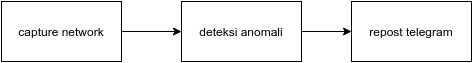
\includegraphics{gambar/gambaranUmum}
	\caption{Gambaran Umum Sistem}
	\label{Gambaran Umum Sistem}
\end{figure}

	\subsection{\emph{(Capture Network)}}
		Pada proses ini akan dilaukan monitoring \emph{traffik} menggunakan \emph{scappy} , setiap semua \emph{traffik} yang berjalan pada \emph{network} akan disamanakan dengan \emph{rule} deteksi yang sudah disediakan selama proses ini tidak akan dilakukan perintah apapun pada sisi \emph{server}. 
	\subsection{Deteksi \emph{Anomali}}
		Pada proses ini dilakukan pemindaian pada \emph{traffik} dan \emph{rule} deteksi yang digunakan, ketika \emph{traffik} tersebut sama dengan \emph{rule} serangan , maka akan terdeteksi sebagai anomali / serangan. Pada proses ini akan mengu perintah untuk melakukan bloking dari telegram.
		
	\subsection{Repost Telegram}
		Proses ini akan mengirim repost berupa pesan ,ketika terjadi anomali/serangan pada \emph{network} dan akan menunggu printah dari user untuk melakukan bloking dan sebagainya.
		
		
	
\section{Gambaran Khusus}


\begin{figure}[H]
	\centering
	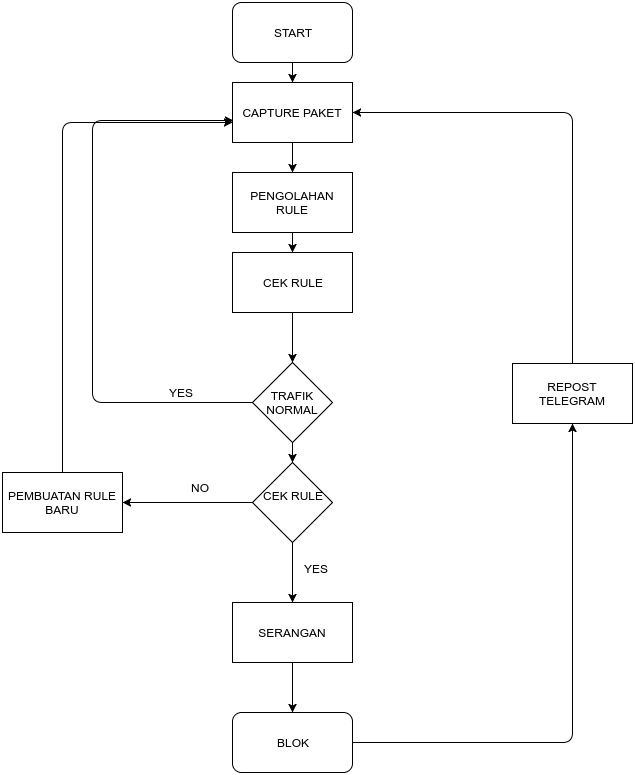
\includegraphics[scale = 0.9 ]{gambar/gambaranKhusus}
	\caption {Gambaran Khusus Sistem}
	\label{Gambaran Khusus Sistem }
\end{figure}

	\subsection{\emph{Capture Packet}}
	Pada proses ini akan dilaukan monitoring \emph{traffik} menggunakan \emph{scappy} , setiap semua \emph{traffik} yang berjalan pada \emph{network} akan disamanakan dengan \emph{rule} deteksi yang sudah disediakan selama proses ini tidak akan dilakukan perintah apapun pada sisi \emph{server}. 

	\subsection{Pengolahan \emph{Rule}}
	Proses ini akan melakukan pengolahan \emph{rule} yang digunakan untuk mendetesi serangan , setiap \emph{rule} yang terbentuk akan disimpan dalam sebuah file yang akan digunakan untuk deteksi anomali
	\subsection{Pemindain \emph{Rule}}
	Pada proses ini dilakukan pemindaian pada \emph{traffik} dan \emph{rule} deteksi yang digunakan, ketika \emph{traffik} tersebut sama dengan \emph{rule} serangan , maka akan terdeteksi sebagai anomali / serangan. Pada proses ini akan mengu perintah untuk melakukan bloking dari telegram.
	
	\subsection{\emph{Blocking}}
	Proses ini akan melakukan perintah dari user melalui telegram , pada proses ini blocking menggunakan tools iptables yang berfungsi sebagai tools untuk melakukan blok paket dan koneksi yang terhadi.
	
	\subsection{Repost Telegram}
	Proses ini akan mengirim repost berupa pesan ,ketika terjadi anomali/serangan pada \emph{network} dan akan menunggu printah dari dari user untuk melakukan bloking dan sebagainya.
	
	\subsection{Pembuatan \emph{Rule} Baru}
	Pada proses pembuatan \emph{rule} baru ini akan dilakukan ketika ada anommali dalam \emph{network} namum \emph{traffik} tersebut tidak terdeteksi sebagai serangan, sehingga dibutuhkan \emph{rule} baru untuk mendeteksi jenis \emph{traffik} tersebut.
\section{\emph{Capture Packet}}
Dalam Penelitian tugas akhir menggunakan fitur packet yang telah disesuaikan
dengan fitur pengoalahan \emph{rule} sebelumnya, yaitu dengan menggunakan dataset hasil
pengolahan dari capture scapy.

\section{Pengolahan \emph{Traffik}}
Pada pengoalahan trafik dilakukan proses pencocokan dengan hasil pengolah-
an dataset serangan yang telah didapatkan.

\begin{table}[H]
	\centering

	
	\caption{\ Jumlah dataset}
	\label{Jumlah dataset}
	\begin{tabular}{|c|l|l|}
		\hline
		NO & \emph{traffik}     & JUMLAH DATASET \\ \hline
		1  & SCANNING    & 5.000.000      \\ \hline
		2  & BRUTE FORCE & 5.000.000      \\ \hline
		3  & DDoS        & 5.000.000      \\ \hline
		4  & NORMAL      & 5.000.000      \\ \hline
	\end{tabular}
\end{table}

\section{Dataset}
Pada penelitian tugas akhir ini diguanakan dataset scapy. Berikut adalah fitur
dataset scapy antara lain:

	
\begin{enumerate}[A.]
	\begin{singlespace}
		\itemsep0em
		\item \emph{Transmission Control Protocol (TCP)}
		\item \emph{Internet Control Message Protocol (ICMP)}
		\item \emph{Internet Protocol Address (IP)}
		\item \emph{User Datagram Protocol (UDP)}

	\end{singlespace}
\end{enumerate}

berikut adalah penjelasan dari masing masing dataset yang digunakan untuk pembuatan \emph{rule} deteksi serangan .

	\newpage
	\subsection{\emph{Transmission Control Protocol (TCP)}}
	\emph{Transmission Control Protocol (TCP)} adalah suatu protokol yang berada di
	lapisan transport (baik itu dalam tujuh lapis model referensi OSI atau model DARPA)
	yang berorientasi sambungan (connection-oriented) dan dapat diandalkan (reliable).
	TCP dispesifikasikan dalam RFC 793.Pada scapy terdapat 11 fitur sebagai berikut : 
	
	\begin{table}[H]
		\centering
		\caption{\ Fitur ICMP}
		\label{Fitur ICMP}
		\begin{tabular}{|l|l|l|}
			\hline
			NO & FITUR     & TIPE \\ \hline
			1  & SPORT    & ShortEnumField      \\ \hline
			2  & DPORT & ShortEnumField      \\ \hline
			3  & SEQ        & IntField      \\ \hline
			4  & ACK      & IntField      \\ \hline
			5  & DATAOFS    & BitField      \\ \hline
			6  & RESERVED & BitField      \\ \hline
			7  & FLAGS        & FlagsField      \\ \hline
			8  & WINDOW      & ShortField     \\ \hline
			9  & CHKSUM    & XShortField      \\ \hline
			10  & ARGPTR &  ShortField      \\ \hline
			11  & OPTIONS        & TCPOptionsField      \\ \hline
		
		\end{tabular}
	\end{table}


	\newpage
	\subsection{\emph{Internet Control Message Protocol (ICMP)}}
	
	 Internet Control Message Protocol (ICMP) adalah salah satu protokol inti dari
	 keluarga protokol internet. ICMP utamanya digunakan oleh sistem operasi komputer
	 jaringan untuk mengirim pesan kesalahan yang menyatakan, sebagai contoh, bahwa
	 komputer tujuan tidak bisa dijangkau.
	 ICMP berbeda tujuan dengan TCP dan UDP dalam hal ICMP tidak digunak-
	 an secara langsung oleh aplikasi jaringan milik pengguna. salah satu pengecualian
	 adalah aplikasi ping yang mengirim pesan ICMP Echo Request (dan menerima Echo
	 Reply) untuk menentukan apakah komputer tujuan dapat dijangkau dan berapa lama
	 paket yang dikirimkan dibalas oleh komputer tujuan. Berikut adalah fitur icmp yang
	 terdapat pada scapy :
	 
	 
	 	\begin{table}[H]
	 	\centering
	 	\caption{\ Fitur ICMP}
	 	\label{Fitur ICMP}
	 	\begin{tabular}{|l|l|l|}
	 		\hline
	 		NO & FITUR     & TIPE \\ \hline
	 		1  & TYPE    & ByteEnumField      \\ \hline
	 		2  & CODE & MultiEnumField      \\ \hline
	 		3  & CHKSUM        & XShortField      \\ \hline
	 		4  & ID      & ConditionalField      \\ \hline
	 		5  & SEQ    & ConditionalField      \\ \hline
	 		6  & TSORI & ConditionalField      \\ \hline
	 		7  & TSRX        & ConditionalField      \\ \hline
	 		8  & TSTX      & ConditionalField     \\ \hline
	 		9  & GW    & ConditionalField      \\ \hline
	 		10  & PTR & ConditionalField      \\ \hline
	 		11  & RESERVED        & ConditionalField      \\ \hline
	 		12 & ADDRMASK	&  ConditionalField \\ \hline
	 		13 & UNUSED & ConditionalField \\ \hline
	 	\end{tabular}
	 	\end{table}
 	\newpage
 	\subsection{\emph{Internet Protocol Address (IP)}}
    	Internet Protocol Address (IP) adalah protokol lapisan jaringan (network la-
 	yer dalam OSI Reference Model) atau protokol lapisan internetwork (internetwork
 	layer dalam DARPA Reference Model) yang digunakan oleh protokol TCP/IP untuk
 	melakukan pengalamatan dan routing paket data antar host-host di jaringan kompu-
 	ter berbasis TCP/IP. Versi IP yang banyak digunakan adalah IP versi 4 (IPv4) yang
 	didefinisikan pada RFC 791 dan dipublikasikan pada tahun 1981, tetapi akan digan-
 	tikan oleh IP versi 6 pada beberapa waktu yang akan datang.Berikut adalah fitur yang
 	terdapat pada IP : 
 	
 	\begin{table}[H]
 		\centering
 		\caption{\ Fitur IP}
 		\label{Fitur IP}
 		\begin{tabular}{|l|l|l|}
 			\hline
 			NO & FITUR     & TIPE \\ \hline
 			1  & VERSION    & BitField      \\ \hline
 			2  & IHL & BitField      \\ \hline
 			3  & TOS        & XByteField      \\ \hline
 			4  & LEN      & ShortField      \\ \hline
 			5  & ID    & ShortField      \\ \hline
 			6  & FLAGS & FlagsField      \\ \hline
 			7  & FRAGS        & BitField      \\ \hline
 			8  & TTL      & ByteField     \\ \hline
 			9  & CHKSUM    & XShortField      \\ \hline
 			10  & SRC &  Emph      \\ \hline
 			11  & DST        & Emph      \\ \hline
 			12 & OPTIONS & PacketListField \\ \hline
 		\end{tabular}
 	\end{table}
 	
 	\subsection{\emph{User Datagram Protocol (UDP)}}
 	User Datagram Protocol merupakan bagian dari internet protocol. Dengan
 	UDP, aplikasi komputer dapat mengirimkan pesan kepada komputer lain dalam ja-
 	ringan lain tanpa melakukan komunikasi awal.[7]
 	UDP melakukan komunikasi secara sederhana dengan mekanisme yang sa-
 	ngat minimal. Ada proses checksum untuk menjaga integritas data. UDP digunakan
 	untuk komunikasi yang sederhana seperti \emph{query DNS (Domain Name System), NTP
 	 	(Network Time Protocol), DHCP (Dinamic Host Configuration Protocol), dan RIP
 	 	(Routing Information Protocol).}
 	

 
 

 \section{\emph{Autonomous System}}
 Cara kerja \emph{Autonomus System} ini adalah ketika \emph{traffik} terindikasi bukan \emph{traffik}
 normal, maka akan dilakukan pemindaian pada jenis serangan pada \emph{rule} yang telah
 disediakan, namun tidak semua \emph{rule} tersebut akan dianggap serangan. Pada kenyata-
 annya \emph{traffik} yang tidak terindikasi serangan ini merupakan serangan jenis lain yang
 dimana didalam \emph{rule} tersebut \emph{traffik} atau ciri ciri serangan ini belum ada. Oleh kere-
 na itu pada penelitian tugas akhir ini dibuat Autonomus System yang dimana \emph{traffik}
 serangan jenis baru secara langsung akan diolah menjadi \emph{rule} baru. Sehingga secara
 terus menerus akan mampu mengenali serangan tipe baru.
 Berikut adalah \emph{flowchart} Autonomus System :
 
 \begin{figure}[H]
 	\centering
 	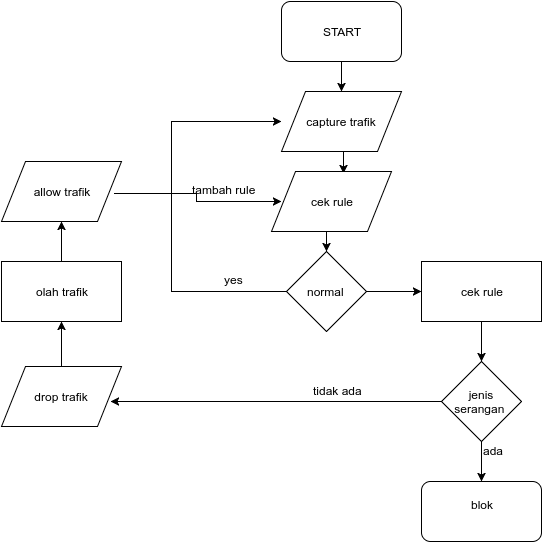
\includegraphics[scale = 0.8]{gambar/autonomusSystem}
 	\caption{Autonomous System}
 	\label{Autonomous System}
 \end{figure}
 
 
 
 \section{\emph{Telegram Command and Control (CNC)}}
 Telegram bot berfungsi sebagai \emph{Command and Control (CNC)} pada bagian ini
 aplikasi telegram berfungsi sebagai kimunikasi antara \emph{server} dan client. Ketika \emph{server}
 mendapat serangan , \emph{server} akan melakukan authentikasi melalui telegram ,sehingga
 sysadmin bisa melakukan tindakan defensive terhadap serangan tersebut berikut adalah gambar \emph{repost telegram}:
 
 
  \begin{figure}[H]
 	\centering
 	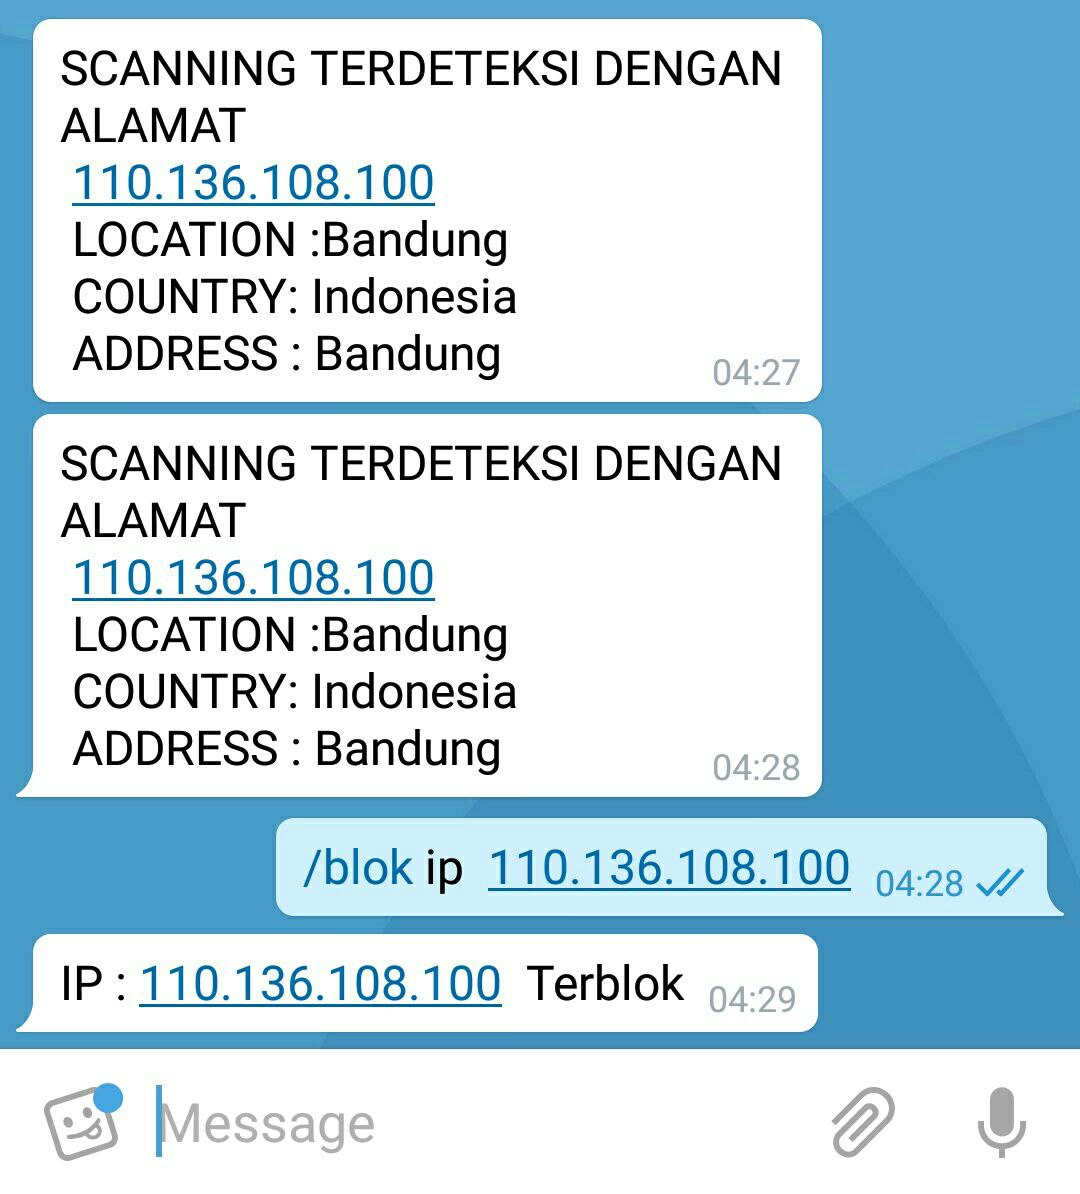
\includegraphics[scale = 0.15 ]{gambar/telegram_bot}
 	\caption{Telegram Repost}
 	\label{Telegram Repost}
 \end{figure}
 
  Berikut adalah \emph{flowchart} TelegramBot

 \begin{figure}[H]
	\centering
	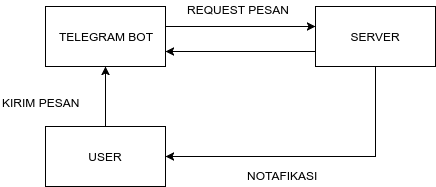
\includegraphics[scale = 0.7 ]{gambar/TELEGRAM}
	\caption{Telegram}
	\label{Telegram}
\end{figure}

Pada flowchrat diatas dapat deketahui \emph{user} mengirim pesan ketelegram , kemuadi setiap pesan akan dianggap sebuah perintah ketika pesan yang dikirimkan dikenali olah \emph{server} , setiap \emph{server} menerima serangan , pesan akan dikirim melalu telegram chat oleh bot ke user.
\section{\emph{Attacking Tools}}
Pada penelitian tugas akhir ini digunakan \emph{tools} untuk  melakukan \emph{attacking} sebagai berikut :


\subsection{NMAP}
\emph{NMAP (Network Mapper)} adalah sebuah aplikasi atau tool yang berfungsi untuk melakukan port \emph{scanning}. Aplikasi ini digunakan untuk meng-audit jaringan yang ada. Dengan menggunakan \emph{tools} ini, kita dapat melihat \emph{host} yang aktif, port yang terbuka, Sistem Operasi yang digunakan, dan \emph{feature-featur scanning} lainnya.

\subsection{NESSUS}
 
Nessus adalah scanner keamanan jaringan yang harus digunakan oleh administrator system . Nessus adalah software yang gratis dan bebas di download. Nessus merupakan sebuah software , yangdapat digunakan untuk meng-audit kemanan sebuah sistem, seperti vulnerability, misconfiguration,security patch yang belum diaplikasikan, default password, dan denial of service.

Nessus berfungsi untukmonitoring lalu-lintas jaringan.Dikarenakan fungsi dari Nessus dapat digunakan untuk mendeteksi adanya kelemahan ataupun cacatdari suatu sistem maka Nessus menjadi salah satu tool andalan ketika melakukan audit keamanan suatusistem. 

\subsection{METASPLOIT AUXILIARY}
Metasploit Auxiliary adalah sebuah tools yang diguanakan untuk melakukan penetrasi keamanan jaringan dengan memamfaatkan celah keaman yang ada , \emph{tools} ini suda dilengkapi dengan \emph{auxiliary} yang berfungsi sebagai tools tambahan untuk melakuan pemindaian pada jaringan yang bertujuan untuk menemukan celah pada jaringan sebelum diexploitasi.

\subsection{TCP Scanning}
Tools ini digunakan untuk melakukan pemindain pada sebuah jaringan yang bertujuan untuk mengetahui \emph{host} yang aktif dan tools ini juga bisa digunakan untuk melakukan pemindain \emph{port} pada \emph{host} yang aktip.

\subsection{HYDRA dan Medusa}
Hydra dan Medusa adalah sebuah tools yang didesain untuk melakukan \emph{brute force} pada sebuah \emph{service} yang membutuhkan \emph{authentication} berupa inputan login untuk dapat melaukan akses.

\subsection{Zero Brute}
Zero brute adalah sebauah tools yang digunakan untuk melakukan serangan \emph{brute force} yang bertujuan untuk mendapatkan hak akses secara penuh pada sebuah titik layanan.

\subsection{Metasploit SynFlood}
Metasploit Auxiliary adalah sebuah tools yang diguanakan untuk melakukan penetrasi keamanan jaringan dengan memamfaatkan celah keaman yang ada , \emph{tools} ini suda dilengkapi dengan \emph{auxiliary} yang berfungsi sebagai tools tambahan untuk melakuan pemindaian pada jaringan yang bertujuan untuk menemukan celah pada jaringan sebelum diexploitasi.

\subsection{Slowloris}
Slowloris adalah sebuah tools DDoS yang berfungsi sebagai alat untuk membanjiri lalu lintas jaringan sehingga bisa membuat layanan tidak bisa berfungsi dengan normal 

\subsection{HULK}
Tools ini didesain untuk membanjiri layanan HTTP dan HTTPS yang berfungsu sebagai titik layanan pada sebuah \emph{web server} , tool ini sering digunakan sebagai DDoS Bot

\subsection{PyLoris}
Tools ini hasil pengembangan dari \emph{slowloris} , tools ini bersifat open-source sehingga kita bisa mengatur layanan yang akan diserangan , biasanya tools ini diguanakan untuk menyerang layanan UDP .

\section{Alat dan Bahan}
	Alat dan bahan yang digunakan pada penelitian ini terbagi atas perangkat keras dan perangkat lunak yang akan dijelaskan seperti berikut.

	\subsection{Perangkat Keras}
	Adapaun perangakat keras yang kami gunakan pada peneletian kali ini adalah
	sebagai berikut

		\vspace{-0.5cm}

		\begin{enumerate}[a.]
		\begin{singlespace}
		\itemsep0em
			\item 1 buah server vps 
			\item 2 unit PC.
			\item 1 buah switch koneksi local (LAN)
			\item kabel LAN RJ45,
			\item 1 buah handphone,
		
		\end{singlespace}
		\end{enumerate}

	\subsection{Perangkat Lunak}
	Adapaun perangakat keras yang kami gunakan pada peneletian kali ini adalah
	sebagai berikut :

		\vspace{-0.5cm}

		\begin{enumerate}[a.]
		\begin{singlespace}
		\itemsep0em
			\item python compiler.
			\item module scapy.
			\item wireshark.
			\item mongodb.
			\item telegram.
			\item Linux Server.
			\item driffnet.
			\item etherape.
			\item nmap 
			\item metasploit 
			\item nessus 
			\item tcp scanning
	.
		\end{singlespace}
		\end{enumerate}


\begin{comment}
\bibliography{daftar-pustaka}
\end{comment}
